\section{About LibrePCB}

\begin{frame}{\secname}
  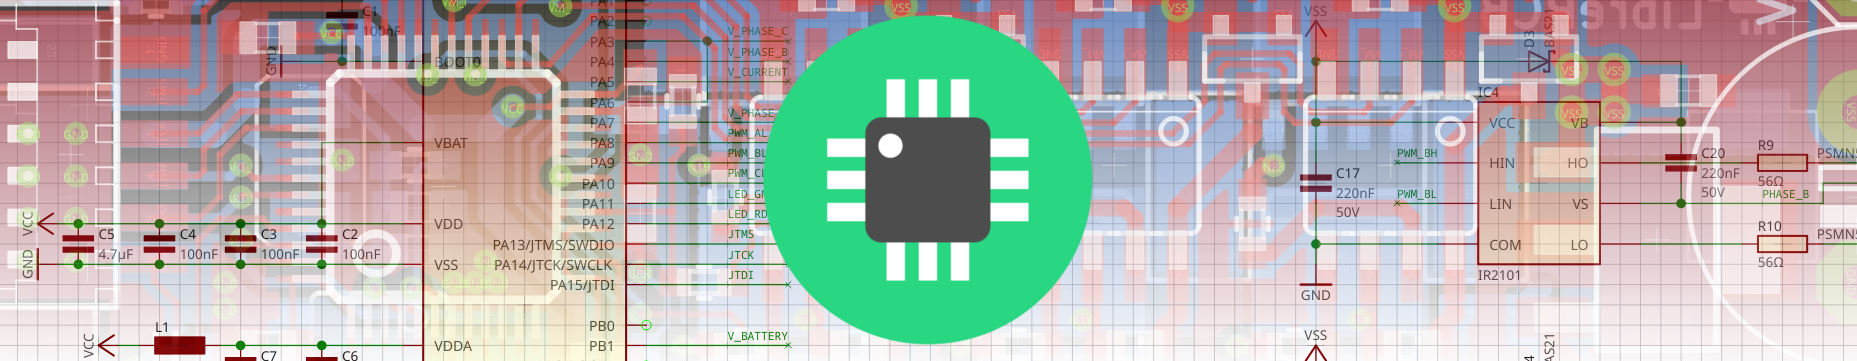
\includegraphics[width=\linewidth]{images/about_header.png}
  \linebreak\linebreak
  \textbf{Free (GPLv3) EDA suite, started in 2013}
  \begin{itemize}
    \item Cross-platform: \faWindows\ \faApple\ \faLinux\ \faFreebsd
          \hspace{0.3em} $|$ x86/ARM/M1
    \item Intuitive \& easy-to-use UI,
          {\footnotesize for beginners, hobbyists \& professionals}
    \item Powerful library concept,
          {\footnotesize to save time and maximize reusability}
    \item Human readable file format,
          {\footnotesize optimized for version control}
    \item Focus on usability and stability
          {\footnotesize rather than bleeding-edge features}
  \end{itemize}
\end{frame}

\note{
  For those who do not know LibrePCB yet, it's an open-source software to
  draw schematics and design PCBs.\\

  It is cross platform and runs on almost every computer - Windows, Linux, macOS
  and more.\\

  It's main goal is to make creating hardware easy, efficient and foolproof
  with an intuitive user interface and powerful architectural concepts.\\

  While the intuitive UI is especially helpful for beginners, it is also
  intended for professional users which care about things like a sane file
  format or a command-line interface to automate tasks.
}
